\documentclass[11pt,a4paper]{article}
\usepackage[margin=2.2cm]{geometry}
\usepackage[T1]{fontenc}
\usepackage{lmodern}
\usepackage{amsmath,amssymb}
\usepackage{booktabs}
\usepackage{tabularx}
\usepackage{float}
\usepackage{enumitem}
\usepackage{xcolor}
\usepackage{tikz}
\usetikzlibrary{arrows.meta,positioning,calc}
\usepackage{caption}
\usepackage{hyperref}
\hypersetup{colorlinks=true, linkcolor=blue!60!black, urlcolor=blue!60!black}

\title{AI651 Assignment 2 -- Question 1\\River Forecasting Proposal}
\date{Fall 2026}

\begin{document}
\maketitle

\paragraph{Proposal in brief.}
We propose a \emph{lag-aware directed spatio-temporal graph network} (LADS-GNN). Every data
source is encoded on its own clock by a causal temporal encoder and projected to a common
width $d$. The sources are then combined on a directed graph that follows the river: reservoir
$\to$ S1 $\to$ S2 $\to$ S3 $\to$ S4, with the monitored tributary T1 joining S2 and a
\emph{latent} node U standing for the unmonitored tributary that joins S3. Upstream information
reaches a station through \emph{delay attention}, a soft choice over a physically bounded range of
travel times whose weights depend on the current flow state, so variable travel times are learned
rather than hard-coded. Every station is linked directly to every upstream source, so information
from the reservoir can reach S4 in a single layer. Announced releases enter as known future inputs.
For S1--S4, the model predicts the level one hour ahead as three quantiles (10\,\%, 50\,\%, 90\,\%)
and is trained with a pinball loss. It has $\approx$0.3\,M parameters, and one forecast takes
milliseconds on a CPU, far inside the 10-minute cycle.

%----------------------------------------------------------------------
\section{Architecture diagram}
%----------------------------------------------------------------------
\begin{figure}[H]
\centering
\resizebox{\textwidth}{!}{%
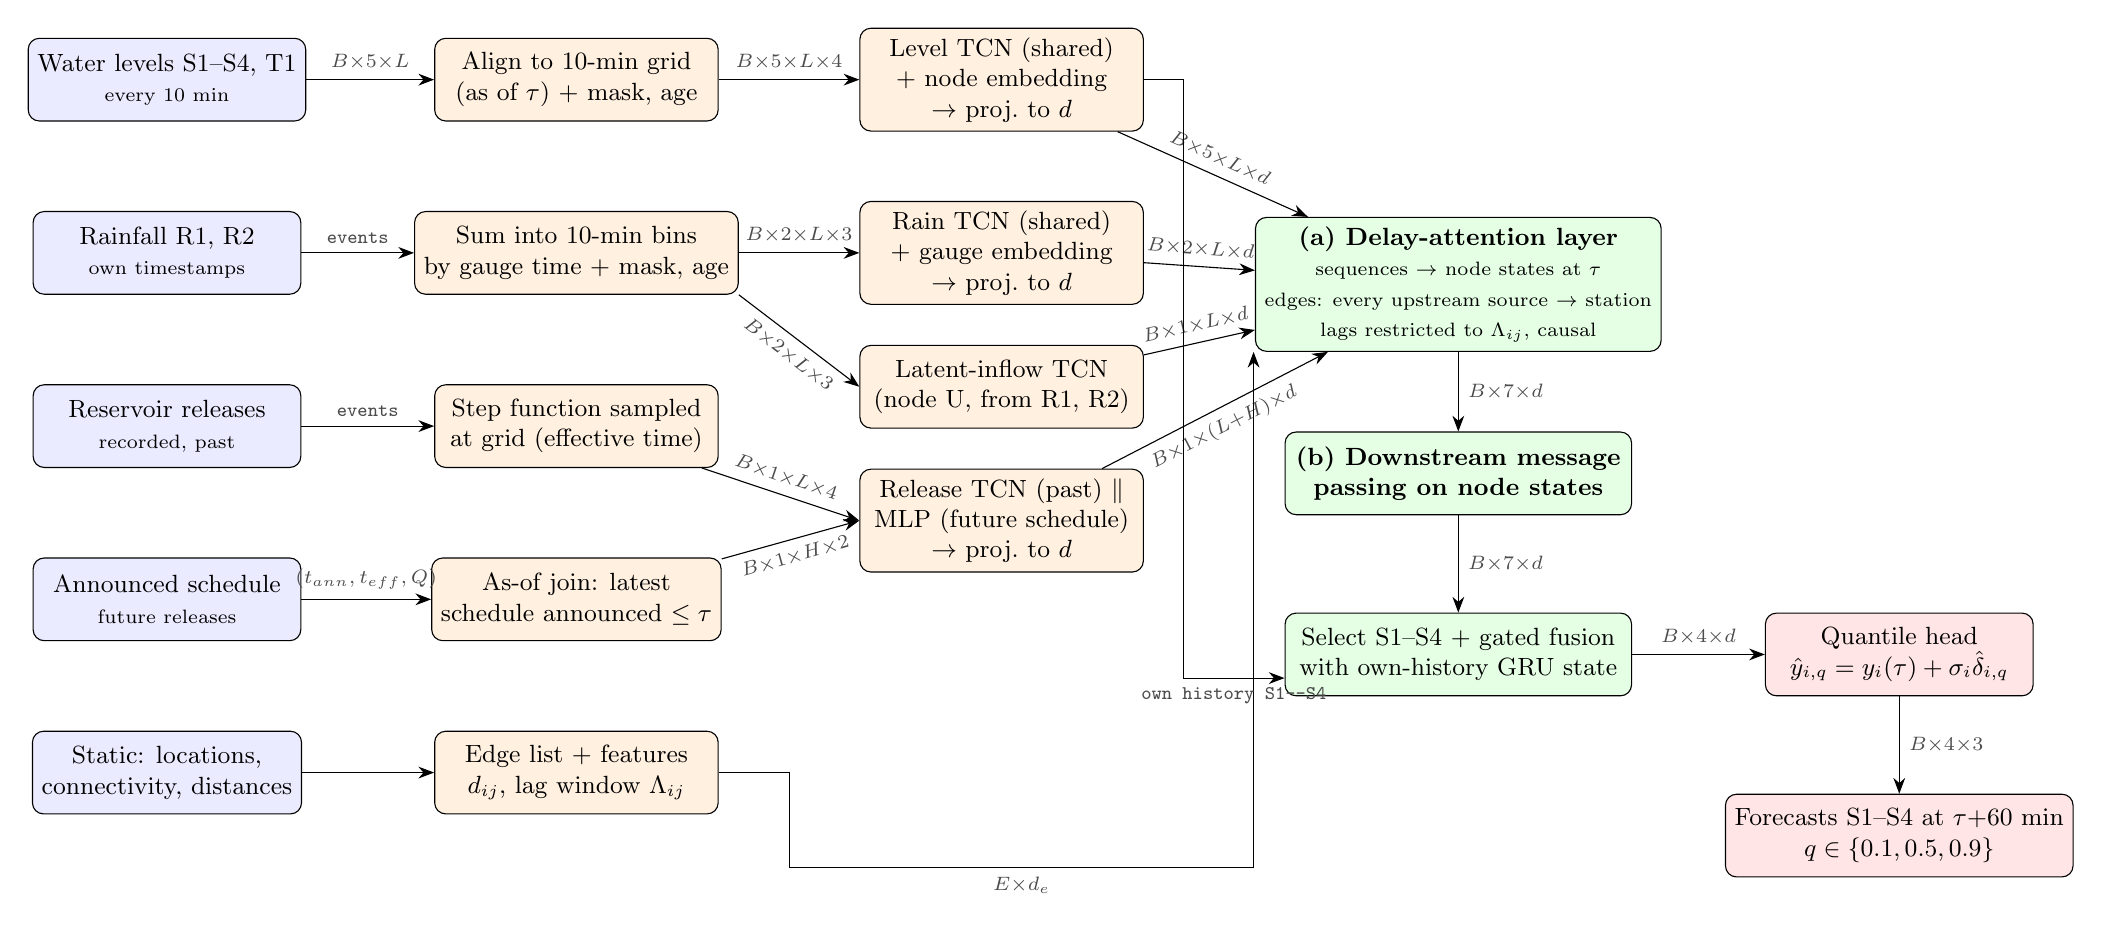
\begin{tikzpicture}[
  font=\small,
  src/.style={draw, rounded corners, fill=blue!8, align=center, minimum width=3.4cm, minimum height=1.05cm},
  blk/.style={draw, rounded corners, fill=orange!12, align=center, minimum width=3.6cm, minimum height=1.05cm},
  gnn/.style={draw, rounded corners, fill=green!10, align=center, minimum width=4.4cm, minimum height=1.05cm},
  outbox/.style={draw, rounded corners, fill=red!10, align=center, minimum width=3.4cm, minimum height=1.05cm},
  dim/.style={font=\scriptsize\ttfamily, text=black!70},
  >={Stealth[length=2mm]}]
% data sources
\node[src] (lev) at (0,0)     {Water levels S1--S4, T1\\\scriptsize every 10 min};
\node[src] (rain) at (0,-2.2) {Rainfall R1, R2\\\scriptsize own timestamps};
\node[src] (rel) at (0,-4.4)  {Reservoir releases\\\scriptsize recorded, past};
\node[src] (sch) at (0,-6.6)  {Announced schedule\\\scriptsize future releases};
\node[src] (sta) at (0,-8.8)  {Static: locations,\\connectivity, distances};
% alignment
\node[blk] (al1) at (5.2,0)     {Align to 10-min grid\\(as of $\tau$) + mask, age};
\node[blk] (al2) at (5.2,-2.2)  {Sum into 10-min bins\\by gauge time + mask, age};
\node[blk] (al3) at (5.2,-4.4)  {Step function sampled\\at grid (effective time)};
\node[blk] (al4) at (5.2,-6.6)  {As-of join: latest\\schedule announced $\le\tau$};
\node[blk] (al5) at (5.2,-8.8)  {Edge list + features\\$d_{ij}$, lag window $\Lambda_{ij}$};
% encoders (each ends with a linear projection to width d)
\node[blk] (enc1) at (10.6,0)    {Level TCN (shared)\\+ node embedding\\$\to$ proj.\ to $d$};
\node[blk] (enc2) at (10.6,-2.2) {Rain TCN (shared)\\+ gauge embedding\\$\to$ proj.\ to $d$};
\node[blk] (encu) at (10.6,-3.9) {Latent-inflow TCN\\(node U, from R1, R2)};
\node[blk] (enc3) at (10.6,-5.6) {Release TCN (past) $\Vert$\\MLP (future schedule)\\$\to$ proj.\ to $d$};
% graph
\node[gnn] (graph) at (16.4,-2.6) {\textbf{(a) Delay-attention layer}\\\scriptsize sequences $\to$ node states at $\tau$\\
  \scriptsize edges: every upstream source $\to$ station\\\scriptsize lags restricted to $\Lambda_{ij}$, causal};
\node[gnn] (mp) at (16.4,-5.0) {\textbf{(b) Downstream message}\\\textbf{passing on node states}};
\node[gnn] (fuse) at (16.4,-7.3) {Select S1--S4 + gated fusion\\with own-history GRU state};
% outputs
\node[outbox] (head) at (22.0,-7.3) {Quantile head\\$\hat y_{i,q}=y_i(\tau)+\sigma_i\hat\delta_{i,q}$};
\node[outbox] (fc) at (22.0,-9.6) {Forecasts S1--S4 at $\tau{+}60$ min\\$q\in\{0.1,0.5,0.9\}$};
% arrows
\draw[->] (lev) -- node[above, dim]{$B{\times}5{\times}L$} (al1);
\draw[->] (rain) -- node[above, dim]{events} (al2);
\draw[->] (rel) -- node[above, dim]{events} (al3);
\draw[->] (sch) -- node[above, dim]{$(t_{ann},t_{eff},Q)$} (al4);
\draw[->] (sta) -- (al5);
\draw[->] (al1) -- node[above, dim]{$B{\times}5{\times}L{\times}4$} (enc1);
\draw[->] (al2) -- node[above, dim]{$B{\times}2{\times}L{\times}3$} (enc2);
\draw[->] (al2.south east) -- node[below, dim, sloped]{$B{\times}2{\times}L{\times}3$} (encu.west);
\draw[->] (al3) -- node[above, dim, sloped]{$B{\times}1{\times}L{\times}4$} (enc3.west);
\draw[->] (al4) -- node[below, dim, sloped]{$B{\times}1{\times}H{\times}2$} (enc3.west);
\draw[->] (enc1) -- node[above, dim, sloped]{$B{\times}5{\times}L{\times}d$} (graph);
\draw[->] (enc2) -- node[above, dim, sloped]{$B{\times}2{\times}L{\times}d$} (graph);
\draw[->] (encu) -- node[above, dim, sloped]{$B{\times}1{\times}L{\times}d$} (graph);
\draw[->] (enc3) -- node[below, dim, sloped]{$B{\times}1{\times}(L{+}H){\times}d$} (graph);
\draw[->] (al5.east) -- ++(0.9,0) -- ++(0,-1.2) -| node[pos=0.25, below, dim]{$E{\times}d_e$} ([xshift=-2.6cm]graph.south);
\draw[->] (graph) -- node[right, dim]{$B{\times}7{\times}d$} (mp);
\draw[->] (mp) -- node[right, dim]{$B{\times}7{\times}d$} (fuse);
\draw[->] (enc1.east) -- ++(0.5,0) |- node[pos=0.75, below, dim]{own history S1--S4} ([yshift=-0.3cm]fuse.west);
\draw[->] (fuse) -- node[above, dim]{$B{\times}4{\times}d$} (head);
\draw[->] (head) -- node[right, dim]{$B{\times}4{\times}3$} (fc);
\end{tikzpicture}}
\caption{LADS-GNN. $B$: batch of issuance times $\tau$; $L=72$ history steps (12\,h at
$\Delta=10$\,min); $H=6$ future steps (1\,h); $d=64$ embedding width; $E$: number of directed edges.
\textbf{Alignment:} every source is put on the issuance-anchored grid
$\{\tau-71\Delta,\dots,\tau\}$ (and $\{\tau+\Delta,\dots,\tau+6\Delta\}$ for the announced schedule)
before encoding. \textbf{Projection:} each encoder ends in a linear layer to width $d$, so
sources with different raw features (4, 3, 4 and 2 channels) can be mixed in the graph.
\textbf{Reshaping:} the graph works on 7 nodes (Res, T1, U, S1--S4); the 4 station rows are
selected ($B{\times}7{\times}d\to B{\times}4{\times}d$) and the head outputs 3 quantiles per
station ($B{\times}4{\times}3$). The own-history GRU path (bottom) is taken from the level
encoder for S1--S4. The node graph is shown in Figure~\ref{fig:graph}.}
\label{fig:arch}
\end{figure}

\begin{figure}[H]
\centering
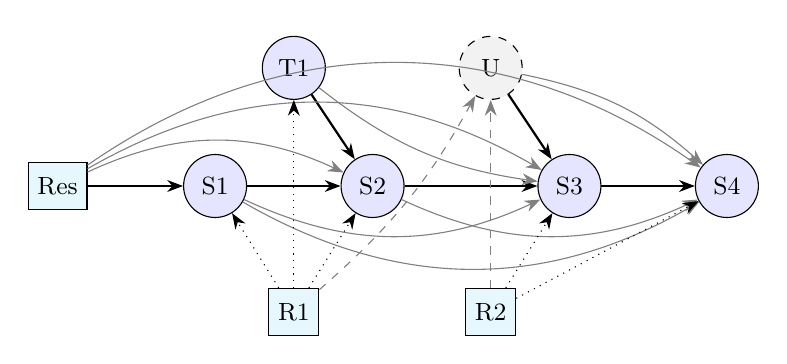
\begin{tikzpicture}[font=\small, >={Stealth[length=2mm]},
  st/.style={circle, draw, fill=blue!10, minimum size=8mm, inner sep=0pt},
  lat/.style={circle, draw, dashed, fill=gray!10, minimum size=8mm, inner sep=0pt},
  rn/.style={rectangle, draw, fill=cyan!10, minimum size=6mm}]
\node[rn] (res) at (0,0) {Res};
\node[st] (s1) at (2,0) {S1};
\node[st] (t1) at (3,1.5) {T1};
\node[st] (s2) at (4,0) {S2};
\node[lat] (u) at (5.5,1.5) {U};
\node[st] (s3) at (6.5,0) {S3};
\node[st] (s4) at (8.5,0) {S4};
\node[rn] (r1) at (3,-1.6) {R1};
\node[rn] (r2) at (5.5,-1.6) {R2};
\foreach \a/\b in {res/s1,s1/s2,t1/s2,s2/s3,u/s3,s3/s4} \draw[->, thick] (\a) -- (\b);
\draw[->, gray, bend left=25] (res) to (s2);
\draw[->, gray, bend left=30] (res) to (s3);
\draw[->, gray, bend left=35] (res) to (s4);
\draw[->, gray, bend right=25] (s1) to (s3);
\draw[->, gray, bend right=30] (s1) to (s4);
\draw[->, gray, bend right=25] (s2) to (s4);
\draw[->, gray, bend right=15] (t1) to (s3);
\draw[->, gray, bend left=15] (u) to (s4);
\draw[->, dotted] (r1) -- (s1); \draw[->, dotted] (r1) -- (s2); \draw[->, dotted] (r1) -- (t1);
\draw[->, dotted] (r2) -- (s3); \draw[->, dotted] (r2) -- (s4);
\draw[->, dashed, gray] (r1) to[bend right=10] (u); \draw[->, dashed, gray] (r2) -- (u);
\end{tikzpicture}
\caption{Directed graph used by the delay-attention layer. Black: physical river links. Grey:
transitive edges from every upstream source to every downstream station, each with its own lag
window, so the reach of one layer covers the whole basin. Dotted: rainfall-to-catchment edges
(initial assignment from gauge locations, A10). Dashed: the latent node U has no sensor, and its
sequence is produced from R1 and R2 by the latent-inflow encoder. All edges point downstream (A7).}
\label{fig:graph}
\end{figure}

%----------------------------------------------------------------------
\section{Assumptions}
%----------------------------------------------------------------------
\textbf{Supplied facts (not assumptions).} 10-minute water levels at S1--S4 and T1; rainfall at
R1 and R2 with timestamps and gauge locations; recorded reservoir releases and announced future
schedules with announcement and effective times; station locations, river connectivity and
along-river distances. A monitored tributary (T1) joins between S1 and S2 and an unmonitored one
between S2 and S3. Stations are unevenly spaced, travel times vary with conditions, precise
travel times and the unmonitored inflow are not supplied, and future rainfall and future levels are
unknown at issuance. Everything below is an assumption made because the brief leaves it open.

\subsection*{Unspecified data conditions}
\begin{description}[leftmargin=0.9cm, style=nextline]
\item[A1 Record length.] At least three years of history are available for all sources and include
several flood seasons. \emph{Why reasonable:} authorities normally keep multi-year telemetry archives.
\emph{Effect on design:} enough events for a small ($\approx$0.3\,M parameter) model, but not for a large
one; data are split chronologically (oldest years train, next season validation, most recent season
test) so that no future information leaks into training.
\item[A2 Reporting delays.] Level telemetry usually arrives within one 10-minute interval but can be up
to 30\,min late; rain gauges report with up to 20\,min delay; reservoir releases are logged within
10\,min. \emph{Why:} typical of radio/GSM telemetry. \emph{Effect:} every input is built ``as of''
$\tau$ with an explicit \emph{age} feature, and training replays these delays (Section~5).
\item[A3 Measurement quality.] Gauges share a common datum; level noise is a few centimetres;
occasional spikes and flat-lines occur. \emph{Why:} standard for pressure/radar gauges.
\emph{Effect:} range and rate-of-change checks flag bad readings, which are then treated as missing.
\item[A4 Missingness.] Gaps are sporadic (a few \% of readings) and occasionally last hours; no
station is missing for most of the record. \emph{Why:} sensors are maintained. \emph{Effect:} masks
plus simple filling suffice; a permanently failed station needs retraining or a fallback model.
\item[A5 Release semantics.] A release value (m$^3$/s) holds from its effective time until the next
record (step function). Announced schedules are usually followed but can be revised or deviate
(gate errors, emergency spills). \emph{Why:} how gate operations are logged. \emph{Effect:} scheduled
and actual releases are separate inputs (Sections~4--5).
\item[A6 Issuance timing.] Forecasts are issued at the grid times
($\ldots$, hh:00, hh:10, $\ldots$) after a short collection cut-off (2\,min), and the target is the
level recorded at $\tau+60$\,min. \emph{Why:} matches the 10-minute logging. \emph{Effect:} defines
$\tau$ and the alignment grid (Section~3).
\end{description}

\subsection*{River dynamics the model assumes}
\begin{description}[leftmargin=0.9cm, style=nextline]
\item[A7 Downstream-only propagation.] There is no tidal influence or significant backwater from
downstream structures on S1--S4. \emph{Why:} an inland river below a reservoir. \emph{Effect:} graph
edges point downstream only, which removes spurious paths and is a strong inductive bias.
\item[A8 Bounded, state-dependent travel times.] The travel time of a flood wave over a distance
$d_{ij}$ is $d_{ij}/c$, with wave celerity $c$ between $c_{\min}=0.5$ and $c_{\max}=4$\,m/s, and $c$
grows with discharge (faster in floods). \emph{Why:} the typical range for lowland and mid-gradient
rivers. \emph{Effect:} edge $j\to i$ may only use lags in
$\Lambda_{ij}=[\lfloor d_{ij}/(c_{\max}\Delta)\rfloor,\ \lceil d_{ij}/(c_{\min}\Delta)\rceil+3]$
(10-minute steps, with a margin). Within $\Lambda_{ij}$ the weights are learned and depend on the
current level (Section~4). Travel time is therefore learned, but physically impossible lags are
excluded.
\item[A9 Smooth, monotone response.] Over one hour, the level change at a station is dominated by
recent upstream changes, routed inflows and local rainfall-runoff. More inflow never lowers the
level downstream. \emph{Why:} mass conservation in an open channel. \emph{Effect:} we predict the
change over persistence (residual form), and an optional penalty keeps the median forecast
non-decreasing in the scheduled release.
\item[A10 Rainfall representativeness.] From the gauge locations, R1 mainly drains to S1, S2 and T1,
and R2 to the unmonitored tributary, S3 and S4. \emph{Why:} nearest-catchment assignment.
\emph{Effect:} initial rainfall-to-node edges. Their weights are learned, so a wrong guess is
down-weighted by the data.
\item[A11 Stationary channel.] No major change of the river bed or the level--flow relation occurs within the
record, and the authority reports such changes. \emph{Why:} short record. \emph{Effect:} one model
for the whole record, with drift monitoring triggering retraining.
\item[A12 Rain after issuance is secondary within one hour.] Rain that has fallen by $\tau$ dominates
the one-hour response, and rain falling after $\tau$ matters mainly for the fastest catchments.
\emph{Why:} runoff concentration times usually exceed one hour. \emph{Effect:} no rainfall forecast
is required, and the remaining effect is absorbed by the upper quantile (Section~6).
\end{description}

%----------------------------------------------------------------------
\section{Forecasting task and data specification}
%----------------------------------------------------------------------
\textbf{Issuance time.} $\tau$ is a 10-minute grid time (A6). A forecast is issued every
$\Delta=10$\,min using only the data that have \emph{arrived} by $\tau$.

\textbf{History window.} $L=72$ steps (12\,h): $\{\tau-71\Delta,\dots,\tau\}$. Twelve hours is longer
than the largest admissible travel time from the reservoir to S4 (A8) plus the rainfall-runoff
response, so the causes of everything that arrives at a station within the next hour lie inside
the window.

\textbf{Horizon.} One hour ahead, i.e.\ $h=6$ steps. The target time is $\tau^{+}=\tau+6\Delta$. The
intermediate steps $\tau+\Delta,\dots,\tau+5\Delta$ are predicted as auxiliary outputs during
training only, to give more training signal. The service publishes $\tau^{+}$.

\textbf{Outputs.} For each station S1--S4, the 10\,\%, 50\,\% (point forecast) and 90\,\% quantiles of the
water level at $\tau^{+}$, in metres above the gauge datum.

\begin{table}[H]
\centering\small
\caption{Inputs and outputs for one batch. $B$ is the batch axis: each sample is one issuance
time $\tau$, and the samples of a batch come from different dates. $L=72$, $H=6$; $E$ is the
number of directed edges.}
\label{tab:data}
\begin{tabularx}{\textwidth}{@{}p{2.6cm}p{2.5cm}Xp{3.6cm}@{}}
\toprule
Tensor & Dimensions & Axis meanings & Time coverage / timestamps\\
\midrule
$\mathbf{Y}^{\mathrm{hist}}$ levels & $B\times5\times L\times4$ & batch; node (S1, S2, S3, S4, T1);
history step; feature (level, 10-min level change, valid mask, age of last valid reading) &
grid times $\tau-71\Delta\ldots\tau$, readings that arrived by $\tau$\\
$\mathbf{P}$ rainfall & $B\times2\times L\times3$ & batch; gauge (R1, R2); history step; feature
(rain in the 10-min bin, valid mask, age) & bins $(\tau-(l{+}1)\Delta,\ \tau-l\Delta]$ by gauge
timestamp, $l=0..71$\\
$\mathbf{Q}^{\mathrm{past}}$ releases & $B\times1\times L\times4$ & batch; reservoir; history step;
feature (actual release, release scheduled for that time, valid mask, age) & grid times
$\tau-71\Delta\ldots\tau$, by effective time\\
$\mathbf{Q}^{\mathrm{sch}}$ schedule & $B\times1\times H\times2$ & batch; reservoir; future step;
feature (scheduled release, time since announcement) & $\tau+\Delta\ldots\tau+6\Delta$ by effective
time; only schedules announced at or before $\tau$\\
$\mathbf{C}$ calendar & $B\times L\times2$ & batch; history step; (sin, cos of day of year) & as history\\
$\mathbf{A}$, $\mathbf{e}$ static graph & $E\times2$, $E\times4$ & edge; (source, target) / edge features
(distance, $\min\Lambda_{ij}$, $\max\Lambda_{ij}$, edge type). Shared by all samples (no batch axis) &
time-invariant\\
\midrule
$\hat{\mathbf{Y}}$ forecast & $B\times4\times3$ & batch; station (S1--S4); quantile (0.1, 0.5, 0.9)
& $\tau^{+}=\tau+6\Delta$\\
$\hat{\mathbf{Y}}^{\mathrm{aux}}$ (training only) & $B\times4\times H\times3$ & batch; station; future
step; quantile & $\tau+\Delta\ldots\tau+6\Delta$\\
$\mathbf{Y}$ target & $B\times4\times H$ (+ mask) & batch; station; future step & $\tau+\Delta\ldots
\tau+6\Delta$ (the service is scored on the last step)\\
\bottomrule
\end{tabularx}
\end{table}

\textbf{Alignment across sampling times.} All sources are mapped onto the same
issuance-anchored grid before encoding.
\begin{itemize}[leftmargin=*,itemsep=1pt]
\item \emph{Levels} (S1--S4, T1) are already on the grid. A slot holds a reading only if the
reading has arrived by $\tau$. Otherwise it is masked and filled with the last valid value, and
its \emph{age} records how stale that value is.
\item \emph{Rainfall} arrives as timestamped events or irregular totals. It is summed into 10-minute bins
by \emph{measurement} time. Bins whose data have not yet arrived are masked.
\item \emph{Releases} are step functions (A5), sampled at each grid time by their \emph{effective}
time. The release that was scheduled for each past time is kept as a second channel, so the network
can see how far the schedule and the actual release have differed.
\item \emph{Announced schedule}: an ``as-of'' join takes, for each future step, the most recent
schedule whose \emph{announcement} time is $\le\tau$. Later announcements are invisible, exactly as
in operation, and a schedule announced before $\tau$ but effective after $\tau+60$\,min is irrelevant.
\end{itemize}

\textbf{Alignment across locations.} Locations are not interpolated onto a spatial grid. Each
sensor is a graph node (S1--S4, T1), or feeds one (R1, R2 feed their catchment nodes and the latent
node U). River geometry enters through the edge features and the lag windows $\Lambda_{ij}$
derived from along-river distances (A8). Encoders are shared across sensors of the same type, a
learned node embedding tells the sensors apart, and per-source linear projections bring every input
to the same width $d$ before the graph layer combines them (Figure~\ref{fig:arch}).

\textbf{Information available at issuance:} all history up to $\tau$ that has arrived, the latest
announced release schedule up to $\tau+60$\,min, and the static data. \textbf{Not available:} future
rainfall, future levels (including any reading not yet delivered), the unmonitored tributary inflow,
and exact travel times.


\end{document}
